\chapter[Title of the chapter 4 displayed \\ in the table of contents]
    {Title of the chapter 4 displayed in the page
        \chaptermark{Ch. 4 title in the header}
    }
    \chaptermark{Ch. 4 title in the header}
\label{ch:labelchapter4}

\updatemylof % to be used with "list of figure divider per chapter" (see PREAMBLE)

\regularsection
\headerregularsection

Author 1\textsuperscript{1,\textcolor{sophia}{$\ast$}}, Author 2\textsuperscript{1,2,\textcolor{sophia}{$\ast$}}, Author 3\textsuperscript{3}, Author 4\textsuperscript{1}, Author 5\textsuperscript{1}, Author 6\textsuperscript{1}, Author 7\textsuperscript{2,4,\#} and Author 8\textsuperscript{1,\#} \hfill \textcolor{sophia}{\textsuperscript{$\ast$}\textit{Author 1 and Author 2 contributed equally to this study.}} \newline

\let\thefootnote\relax\footnotetext{\textsuperscript{1}Department X, University 1, City A, Country B. 
\textsuperscript{2}Department Y, University 2, City C, Country D. 
\textsuperscript{3}Institute E, City F, Country G. 
\textsuperscript{4}Research Center H, University I, City J, Country K. 
\textsuperscript{\#}e-mail: \href{mailto:author7@university2.ac.countryD}{author7@university2.ac.countryD} and \href{mailto:author8@universityI.countryK}{author8@universityI.countryK}}

\noindent First published in: \textit{Scientific Reports} \textbf{10}, 853 (2020). \hfill \break
DOI: \href{https://doi.org/10.1038/s41598-019-55424-z}{10.1038/s41598-019-55424-z} 

\begin{wrapfigure}[3]{l}{0.2\textwidth}
    
\includegraphics[width=0.2\textwidth]{figures/by.png}
\end{wrapfigure} 

\noindent \textcolor{white}{test} \newline \textbf{Open Access} This article is licensed under a Creative Commons Attribution 4.0 International License. It means that unrestricted use, sharing, adaptation, distribution, and reproduction in any medium or format are allowed, as long as the original author(s) and the source are appropriately credited, a link to the Creative Commons license is provided, and any changes made are indicated. To view a copy of this license, please visit \href{http://creativecommons.org/licenses/by/4.0/}{http://creativecommons.org/licenses/by/4.0/}. \newline

\noindent \copyright \ Liudi Mulyo \textit{et al}, 2020. \newline

\noindent \textbf{Contributions} \newline
\noindent \lipsum[2]

%%%%%%%%%%%%%%%%%%%%%%%%%%%%%%%%%%%%%%%%%%%%%%%%%%%%%%%%%%%%%%%%%%%%%%%%%%%%%%%%%%%%%%%%%%%%%%%%%%%%%%%%%%%%%%%%%%%%%%%%%%%

\tcbset{enhanced,colback=abstractback,colframe=sophia,fonttitle=\bfseries}
\begin{tcolorbox}[left=3.35cm,grow to left by=3.5cm,right=3.33cm,grow to right by=3.5cm,title={\normalfont \color{White} \small \fontfamily{bch} \selectfont \scshape Abstract}]
% https://tex.stackexchange.com/questions/232878/inserting-pictures-in-tcolorbox
% https://tex.stackexchange.com/questions/169794/outer-margin-of-tcolorbox/169877
% https://tex.stackexchange.com/questions/11484/how-to-draw-a-frame-box-around-an-arbitrary-large-piece-of-text-figures-whatever
\begin{minipage}[t]{\linewidth}
\vspace*{-29pt}
\phantomsection % to fix wrong hyperref to "Abstract" 
\section*{} % for linking from TOC (only one way)
\addcontentsline{toc}{section}{Abstract}
\begin{sloppypar}
\lipsum[1]
\end{sloppypar}

\end{minipage}

\vspace*{3.5pt}
\end{tcolorbox}

%%%%%%%%%%%%%%%%%%%%%%%%%%%%%%%%%%%%%%%%%%%%%%%%%%%%%%%%%%%%%%%%%%%%%%%%%%%%%%%%%%%%%%%%%%%%%%%%%%%%%%%%%%%%%%%%%%%%%%%%%%%

\begin{sloppypar} % to suppress overfull box

Lorem \index{Lorem} ipsum dolor sit amet, consectetuer adipiscing elit \cite{LIUDIMULYO201767}. Ut purus \index{purus} elit,vestibulum ut, placerat ac, adipiscing vitae, felis \citenum{LIUDIMULYO201767}. Curabitur dictum \index{dictum} gravidamauris. Nam arcu libero, nonummy eget, consectetuer id, vulputate a, magna. Donec vehicula augue eu neque \cite{liudimulyo_2018}. Pellentesque habitant morbi tristique senectuset netus et malesuada fames ac turpis egestas \index{egestas}\citenum{liudimulyo_2018}. Mauris ut leo. Cras viverra metusrhoncus sem \cite{2019liudimulyo}. Nulla et lectus vestibulum urna fringilla ultrices. Phasellus eutellus sit amet tortor gravida placerat \citenum{2019liudimulyo}. Integer sapien est, iaculis in, pretium quis,viverra ac, nunc. Praesent eget sem vel leo ultrices bibendum \cite{liudimulyo2020853}. Aenean faucibus. Morbi dolor nulla, malesuada eu, pulvinar at (\ref{fig:figures/paper-iv/fig-4}), mollis ac, nulla. Curabitur auctorsemper nulla \citenum{liudimulyo2020853}. Donec varius orci eget risus. Duis nibh mi, congue eu, accumsaneleifend, sagittis quis, diam. Duis eget orci sit amet orci dignissim rutrum \cite{LIUDIMULYO201767,liudimulyo_2018,2019liudimulyo,liudimulyo2020853,liudimulyo_unpublished1,liudimulyo_unpublished2}. For more information, see \hyperref[appendix:A]{Appendix A}, specifically in \ref{tab:appendixA}.

\end{sloppypar}

\begin{figure} % \begin{figure} will let LaTeX decide the best figure placement for you ; \begin{figure}[H] for forcing the figure placement here ; in the bottom, \begin{figure}[!b] ; top of the page, \begin{figure}[!t]
    \centering
    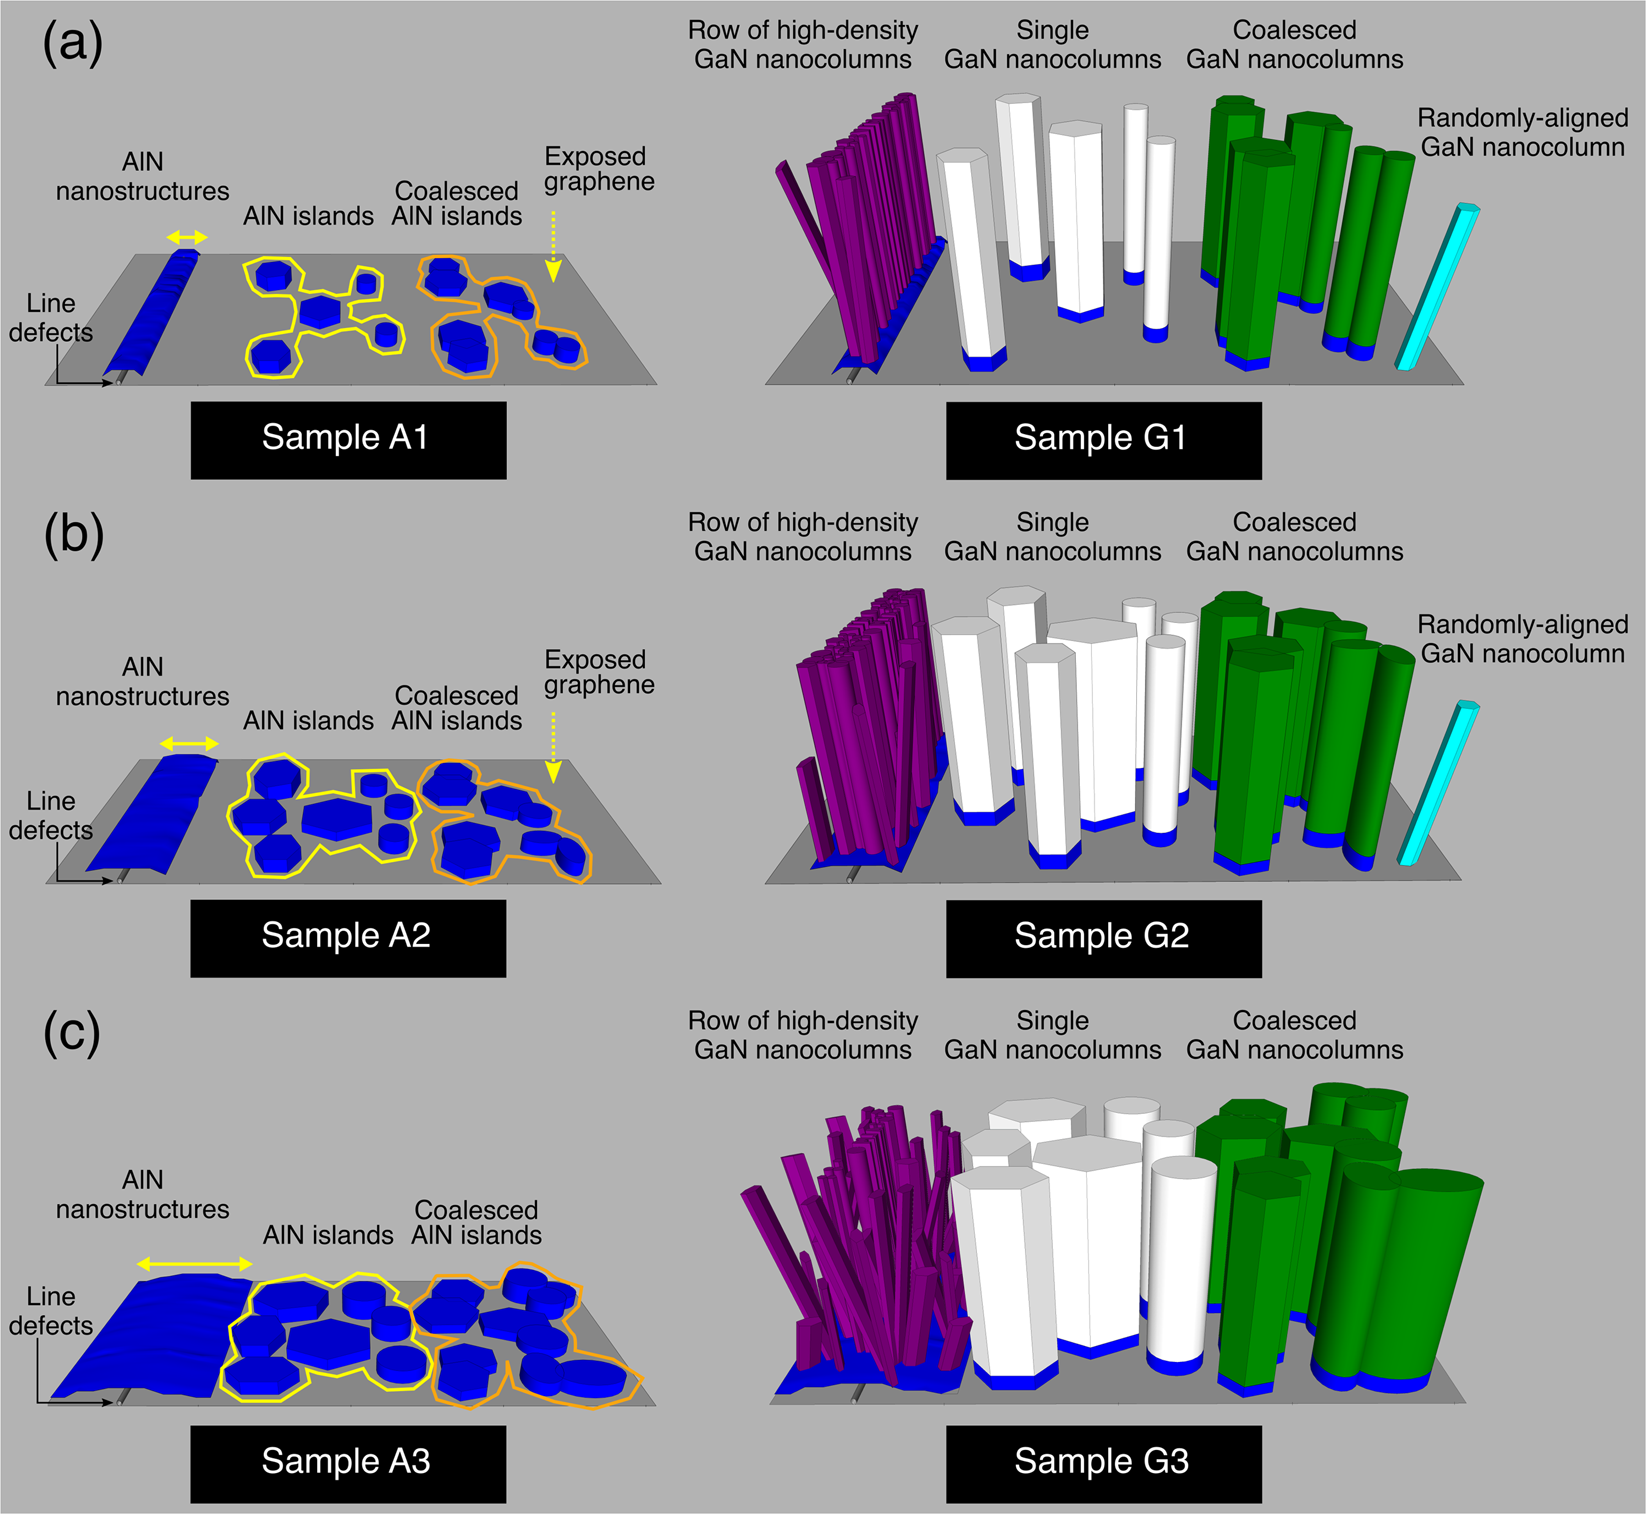
\includegraphics[width=\textwidth]{figures/paper-iv/fig-4.png}
    \caption[Simplified schematics of the AlN buffer structures and GaN nanocolumn formation on graphene]{Simplified schematics of the AlN buffer structures and GaN nanocolumn formation on graphene. Samples (\textbf{a}) A1-G1, (\textbf{b}) A2-G2 and (\textbf{c}) A3-G3. There are two possible AlN (blue) nanostructures forming on graphene: 1) AlN islands and 2) AlN nanostructures along the line defects of graphene (the yellow arrows indicate their lateral growth spread further away from the line defects). Single (white) and coalesced (green) vertical GaN nanocolumn structures are nucleated from the AlN islands, while row of high-density nanocolumns (purple) form on the AlN nanostructures that spread from the line defects. Additional tilted nanocolumns (cyan) are likely to grow on exposed graphene (adapted with permission from ref. \citenum{liudimulyo2020853} \copyright \ Liudi Mulyo \textit{et al}, 2020.}
    \label{fig:figures/paper-iv/fig-4}
\end{figure}

\section{Section 1 in chapter 4}
\lipsum[2-4]

\subsection{Subsection 4.1 of section 1 in chapter 4}
\lipsum[5-7]

\subsection{Subsection 4.2 of section 1 in chapter 4}
\lipsum[8-11]

\clearpage\phantomsection % to fix wrong hyperref to this section
\section[Long section title displayed in the table of content]{Short section title in the chapter}
\sectionmark{Even shorter title on the header}
\lipsum[11-20]

\subsection{Subsection 4.2 of section 2 in chapter 4}
\lipsum[13-14]

%=======================================================================
%%% References 

% \clearpage
\phantomsection
\specialsection % put an indent, see preamble
\headerspecialsection

{\hypersetup{urlcolor=ntnu,linkcolor=sophia} % set clickable URL title color to black, not ntnu like in the main document

\bibliographystyle{unsrtnat-mod}  % NATBIB ref style
\bibliography{references}
}